%%%%%%%%%%%%%%%%%%%%%%%%%%%%%%%%%%%%%%%%%%%%%%%%%%%%%%%%%%%%%%%%%%%%%%%%%%%%%%%

\documentclass[journal]{IEEEtran}

%%%%%%%%%%%%%%%%%%%%%%%%%%%%%%%%%%%%%%%%%%%%%%%%%%%%%%%%%%%%%%%%%%%%%%%%%%%%%%%


% =============================================================================
% Include packages
% =============================================================================

\usepackage[cmex10]{amsmath}  % needed e.g. for align-environment
\usepackage{amssymb}  % needed e.g. for \lesssim
\usepackage{cite}
\usepackage[capitalise]{cleveref}  % auto-prepend Eq., Fig., Tab., etc.
\usepackage[T1]{fontenc}
\usepackage{graphicx}
\usepackage[utf8x]{inputenc}
\usepackage{microtype}  % improves readability and saves space
\usepackage{siunitx}  % for correct typesetting of units, e.g. ohm
%\usepackage{subcaption}
\usepackage{upgreek}  % needed for bold 'micro' sign in abstract
\usepackage{xspace}  % needed for bold 'micro' sign in abstract

\usepackage{tikz}

% =============================================================================
% Own macros
% =============================================================================

% Define dBm as \dbm and re-define dB as \db. This is against the rules of
% siunitx, which prefers defining dB as \deci\bel (hence, dBm would be defined
% as \deci\belm.

\DeclareSIUnit\db{dB}
\DeclareSIUnit\dbm{dBm}

\DeclareSIUnit\MHz{MHz}
\DeclareSIUnit\GHz{GHz}

\newcommand{\boldum}{\,\boldmath$\upmu$m\xspace}  % bold 'um' in abstract

\newcommand{\VDC}{V_\text{DC}}    % DC voltage
\newcommand{\IDC}{I_\text{DC}}    % DC current
\newcommand{\PDC}{P_\text{DC}}    % DC power
\newcommand{\pDC}{p_\text{DC}}    % DC power, normalized
\newcommand{\PRF}{P_\text{RF}}    % fundamental RF power
\newcommand{\pRF}{p_\text{RF}}    % fundamental RF power, normalized
\newcommand{\etaD}{\eta_\text{D}} % drain efficiency

\newcommand{\vB}{v_\text{B}}   % normalized class-B voltage
\newcommand{\Vk}{V_\text{k}}   % knee voltage
\newcommand{\vJ}{v_\text{J}}   % normalized reactive class-J voltage
\newcommand{\vRJ}{v_\text{RJ}} % normalized resistive-reactive class-J voltage

% =============================================================================
% Own setup
% =============================================================================

% setup the graphics path and their extensions so you won't have to specify these 	  with every instance of \includegraphics
\graphicspath{{graphics/}}
\DeclareGraphicsExtensions{.pdf,.jpeg,.png,.pdf_tex}

% font of si units adapted by the font of the environment
\sisetup{detect-all=true}


%%%%%%%%%%%%%%%%%%%%%%%%%%%%%%%%%%%%%%%%%%%%%%%%%%%%%%%%%%%%%%%%%%%%%%%%%%%%%%%


\begin{document}

\title{Investigation and Realisation of a Riemann Pump in 250nm GaN Technology for the Frequency of \SI{100}{\MHz}}

\author{%
	Markus~Wei\ss{},
    Christian~Friesicke,
    R\"{u}diger~Quay,
    and~Oliver~Ambacher\\
    Fraunhofer Institute for Applied Solid State Physics\\
    Freiburg, Germany\\
    markus.weiss@iaf-extern.fraunhofer.de%	markus.weiss@iaf-extern.fraunhofer.de
    %
    \thanks{%
      Manuscript received March 19, 2015;
      revised May 26, 2015;
      accepted July 19, 2015.
      Date of publication Month XX, 2015;
      date of current version July 29, 2015.
      This work was supported and funded by the German Space Management
      (DLR) on behalf of the German Ministry of Economics and Technology (BMWi)
      under research contracts 50YB1128 and 50YB1504.%
    }%
    \thanks{
      C. Friesicke and A.~F. Jacob are with the Institut f\"{u}r
      Hochfrequenztechnik, Technische Universit\"{a}t Hamburg-Harburg, 21073
      Hamburg, Germany (E-mail: cfriesicke@ieee.org).%
    }%
    \thanks{R.~Quay is with the Fraunhofer Institute for Applied Solid-State
      Physics (IAF), 79108 Freiburg, Germany.%
    }%
    \thanks{%
      Color versions of one or more of the figures in this letter are available
      online at http://ieeexplore.ieee.org.}
    \thanks{%
      Digital Object Identifier 10.1109/LMWC.2015.XXXXXXX%
    }%
}

\markboth{IEEE Microwave Wireless and Components Letters,%
          Vol. XX, No. X, Month 20YY}%
         {Friesicke \MakeLowercase{\textit{et al.}}:
          The Resistive-Reactive Class-J Power Amplifier Mode}

\maketitle


% =============================================================================
% Abstract
% =============================================================================

\begin{abstract}
%
A novel architecture for a digital-to-analog converter is investigated, yielding an arbitrary waveform generator.\\%%
\textit{This letter introduces a theory which considers the effect of lossy
second-harmonic terminations on the voltage waveform, output power, and
efficiency of power amplifiers (PAs) operated in the class-J mode. To this end,
the conventional (reactive) class-J mode is extended to a resistive-reactive
class-J mode with complex fundamental and second-harmonic load impedances.
The theory is experimentally validated by performing on-wafer active load-pull
measurements on an AlGaN/GaN HEMT power device with 0.25\boldum gate length and
a total gate periphery of 6$\times$200\boldum. The measured waveforms are
de-embedded to the internal current-generator of the device, where they exhibit
the theoretically predicted behavior.}
%
\end{abstract}
%
\begin{IEEEkeywords}
  AWG, DAC, transmitter architecture.
\end{IEEEkeywords}
%
% =============================================================================
% Introduction
% =============================================================================
%
\section{Introduction}
\label{sec:introduction}
{\itshape \IEEEPARstart{A}{part} from output power and efficiency, research increasingly
focuses on bandwidth as an additional critical parameter of power amplifiers
(PAs) for wireless systems. This results from the higher data rates of current
systems and from the trend towards frequency agility or multi-band operation.
%
Conventional high-efficiency PA modes such as class-B, class-F, or inverse
class-F are not suitable for wideband PA realizations because they require
resonant harmonic loads (open or short circuits). This restriction is overcome
by continuous PA modes such as class-J crippscontinuity2009,
continuous class-F
citecarrubbacontinuous2010,
or continuous inverse class-Fcitecarrubbaexploring2011, friesickemode2011.
%
The class-J mode is based on the class-AB/B mode but adds a reactance to the
fundamental load, which is compensated by a second-harmonic reactance with
opposite sign. It maintains the same efficiency and power as class-AB/B,
however, at the expense of higher peak voltages. Class-J (and the other
continuous modes) rely on purely reactive harmonic loads. Therefore, the
fundamental band (complex loads) can not overlap with the second-harmonic band
(pure reactances). This separation limits the theoretically achievable
bandwidth to 70.7\%. In practice, the transition region between the bands
further reduces the bandwidth. If this region is used, wider bandwidths can be
achieved but lossy harmonic loads must be accepted
cite{preisdesign2014,anderssondecade2012}.
%
Theories that include harmonic losses exist for continuous class-F
cite{carrubbaextension2011}
and continuous inverse class-F
cite{carrubbacontinuous2012}.
This letter presents a theory that considers second-harmonic losses in the
class-J PA mode. The theory is described in \cref{sec:theory}, where the
effects of losses on voltage waveforms, power, and efficiency are calculated,
and the relation between optimum fundamental load and complex second-harmonic
load is derived. \cref{sec:experiment} validates the theory by presenting
on-wafer active harmonic load-pull measurements of a GaN HEMT device.}
%
%
\section{Concept of the Riemann Pump circuit}
\label{sec:theory}
%
In this section a digital-to-analog converter (DAC) is described which is established from the concept of a charge pump.
The digital-to-analog conversion is based on the current steering topology and pumps charges to a capacitive output load.
In dependence on Bernhard Riemann, who founded the Riemann integral, this custom charge pump is named Riemann Pump.
%
\subsection{Idea of the Riemann Pump}
This technique made it possible to synthesize arbitrary signal waveforms, since the output voltage is generated by the integration of different current amplitudes over time at a capacitor, see Equation \ref{eq:current_nomenclature_and_classb}.
%
\begin{align}
  V_{out} =  \frac{1}{C_{out}} \int_0^t \! i_{out}(\tau) \, \mathrm{d}\tau.
    \label{eq:current_nomenclature_and_classb}
\end{align}
%
Absolutely essential to generate different output signals is to establish different current amplitudes to charge and discharge the output capacitor.
%To generate different output signals it is necessary to establish different constant current amplitudes to charge and discharge the capacitor.
Consistent current sources as well as a high sampling frequency were needed to ensure a high signal integrity.
In Fig. \ref{fig:SlopeSynthSignal}(a) eight different slopes represent four different current amplitudes plus their direction times the sampling interval.
These eight slopes correspond to a three bit resolution of the DAC. 
%To explain the concept in a proper way, eight different currents are established which corresponds to a three bit digital-to-analog converter.
Figure \ref{fig:SlopeSynthSignal}(b) illustrates an example of a synthesized output signal using these slopes.
%
% -----------------------------------------------------------------------------
\begin{figure}[htb]
  \centering
	\begin{scriptsize}
  	\def\svgwidth{\columnwidth}
 	\input{graphics/SlopeSynthSignal.pdf_tex} 
  	\caption{(a) Representation of relative slopes and (b) signal generation with riemann code.}
  	\label{fig:SlopeSynthSignal}
	\end{scriptsize}
\end{figure}
% -----------------------------------------------------------------------------
%
%To increase the signal integrity it was also possible to increase the sampling frequency and hence decrease sampling time to synthesize the desired signal.
The solid black line represents a former calculated desired output signal which should be synthesized using the Riemann Pump.
For each sampling point the slope is chosen which minimizes the error between the sampled desired and the synthesized signal.
As the eight slopes are encoded it is possible to control the output signal with a digital input stream representing the sequence of slopes to synthesize the signal.

%
\subsection{Circuit design}
In order to generate these eight different currents the concept of a charge pump in a push-pull configuration is used.
The pushing transistors contribute to an increase of the output signal while the pulling transistors decrease the amplitude of the output signal.
Mandatory for the correct functioning of the push-pull configuration is a digital driver circuit to ensure a proper switching of the transistors connected to the top rail.
% so the pushing transistors switch correctly on/off because they do not have a source grounding.
%To ensure the correct switching of the voltage controlled current source to the top rail a proper driver circuit is needed. 
Figure \ref{fig:schematic_multibit_rp} shows the schematic of the Riemann Pump, where the single stages are cascaded in parallel.
%
% -----------------------------------------------------------------------------
\begin{figure}[htb]
  \centering
	\begin{scriptsize}
  	\def\svgwidth{\columnwidth}
 	\input{graphics/schematic_RP_multibit_smallScale.pdf_tex} 
  	\caption{Schematic of the riemann pump. Marked on the left side is the driver circuit which is necessary. The push-pull stages are/were connected in parallel.}
  	\label{fig:schematic_multibit_rp}
	\end{scriptsize}
\end{figure}
% -----------------------------------------------------------------------------
The dimension of the power transistors in parallel is increased linearly with the power of 2 to ensure the correct encryption by eight bits.
% each higher power transistor is double the size of the former one...
A huge advantage of this technology is, that it is able to provide high power while having an immense switching speed and hence synthesize a signal with high integrity.
In fact of this the load of a the push-pull stage can be implemented as a power amplifier which is directly connected to the antenna for wave propagation.
Therefore much external components are not necessary.
Since the input impedance characteristic of a power transistor is capacitive this is utilized to generate the output signal.
%The load of the described concept consists of the input impedance of a power amplifier which amplifies the signal and propagate it to the antenna.
%The charging and discharging of the capacitive input impedance of the power amplifier led to the possibility to generate arbitrary waveforms.
%% -----------------------------------------------------------------------------
%\section{Output signal simulation of the Riemann Pump}
%\label{sec:simulation}
%% -----------------------------------------------------------------------------
%This section describes the simulation results of the presented concept.
%The circuit used for this simulation is based on the assembled device under test, to ensure proper comparison of the results.
%The simulation confirms the possibility to generate different signals using this concept.
%Figure \ref{fig:input_ctrl_signal} shows the input signal (digital) used to control the DAC.


% -----------------------------------------------------------------------------
\section{Implementation and assembly of a demonstrator}
\label{sec:assembly}
% -----------------------------------------------------------------------------
To the best of the author's knowledge, the first ever built demonstrator is presented to proof the investigated concept.
In order of limited measurement equipment the demonstrator is built with four inputs which corresponds to a two bit resolution.
%The first ever built demonstrator to proof the concept of the Riemann Pump is presented in the following subsection.
For the digital switching of the power transistors a monolithic microwave integrated circuit (MMIC) is used which has already implemented a proper driver circuit and power transistor.
The MMICs are designed and fabricated in the \SI{0.25}{\micro\meter} AlGaN/GaN HEMT technology by Fraunhofer IAF and are of assistance in this realisation of a Riemann Pump, while the conventional application is in a Class-S amplifier (cite Stephan Maroldt).
Figure \ref{fig:assembled_demonstrator} (a) illustrates the schematic where the grey painted area show a single MMIC.
In Fig. \ref{fig:assembled_demonstrator}(b) the layout of the realised demonstrator is illustrated.
%
% -----------------------------------------------------------------------------
\begin{figure}[htb]
  \centering
	\begin{scriptsize}
  	\def\svgwidth{\columnwidth}
 	\input{graphics/circuit_schematic_layout_ddrixy6.pdf_tex} 
  	\caption{(a)Schematic of assembly; grey highlighted the used MMICs. (b) Assembled demonstrator layout.}
  	\label{fig:assembled_demonstrator}
	\end{scriptsize}
\end{figure}
% -----------------------------------------------------------------------------
%
The green shapes represent MIM capacitors for filtering purpose and the black the used MMICs.
In order to reduce the impact of phase delays of the signal the input and output lines are of the same length, as well as the bond wires.
%A critical point/ disadvantage of the used MMICs is that their source potential is led to the backside metallisation to ensure proper heat transfer, while the source potential is on ground.
%The problem in this approach is to drive the power transistor to the upper power rail while the source potential is on the output potential of the ic.
As the used MMICs were processed with backside metallisation and hence the power transistors source potential is grounded, it was necessary to isolate two of the chips.
To ensure that the pushing transistors source potential is connected to the output line of the DAC they were bonded onto an isolated pad to the substrate.
The trade-off which comes with this solution is that the heat transfer is not optimal.\\
%In fact of this the heat transfer is not optimal since the transistors generate several watts.
%Also two different layouts are designed to compare the property of heat transfer.
% Each MMIC used in this work consists of the elements shown in Fig \ref{fig:schematic_multibit_rp} for the low side, which include the driver circuit of two transistors and the resistor plus the output power transistor.
%In fact of the assembly, one version used a isolated pad in fact of the undesired backside metallisation of the chip.
%This is undesired since the output of the high side stage is the source pin.
%For the low side the source pin is grounded and the output is the drain of the power amplifier.
Nevertheless, to the best of the author's knowledge, the first ever realized Riemann Pump in GaN technology were assembled and tested.
Figure \ref{fig:photo_chipconnection_demonstrator}(a) shows a photograph of the bonded chip connection according to the layout in Fig. \ref{fig:assembled_demonstrator}(b).
This chip connection marked with the red shape is illustrated in (b), the photograph of the whole assembled demonstrator.
% -----------------------------------------------------------------------------
\begin{figure}[htb]
  \centering
	\begin{scriptsize}
  	\def\svgwidth{\columnwidth}
 	\input{graphics/PhotoChipConnect_Demonstrator.pdf_tex} 
  	\caption{(a) Chipconnection Photo, (b) realized demonstrator.}
  	\label{fig:photo_chipconnection_demonstrator}
	\end{scriptsize}
\end{figure}
% -----------------------------------------------------------------------------
The demonstrator is of the size 50x60 mm, has four input and one output line and in addition to the DC supply voltage connectors a decoupling network.
%
% ------------------------------------------------------------------------------
\section{Time domain measurement of synthesized output signal compared to simulation}
\label{sec:experiment}
% ------------------------------------------------------------------------------

%The theoretical waveforms are experimentally verified using the demonstrator which is assembled with four MMICs as shown in Figure \ref{fig:assembled_demonstrator} (b). 
% and consists of an input driver stage with a power transistor.
To proof that the built demonstrator can convert digital input streams into an analog output signal the time domain measurement was performed.
For this a special control and measurement strategy was applied.
Four input signals have to be applied to test the two bit resolution of the device. Two differential input signals, hence four signals in total, were applied by an arbitrary waveform generator (Keysight M8195A) to represent a digital data stream. 
These signals had to be amplified by a broadband pre-amplifier and shifted in the DC offset with bias tees to ensure proper switching of the transistors at the input.
%
\subsection{Time domain measurement with resistive load}
First of all a short stability check ensured that the device under test does not oscillate.
Further the switches are controlled with an synchronous signal, as seen in Figure \ref{fig:meas_Input_Output_RLoad_100M_SmallSize_Paper}(a), leading to a push-pull measurement with resistive load.
Hence the output signal switches between Vdd and GND as can be seen in Figure \ref{fig:meas_Input_Output_RLoad_100M_SmallSize_Paper}(b).
%
% -----------------------------------------------------------------------------
\begin{figure}[htb]
  \centering
	\begin{scriptsize}
  	\def\svgwidth{\columnwidth}
 	\input{graphics/meas_Input_Output_RLoad_100M_SmallSize_Paper.pdf_tex} 
  	\caption{(a) Differential input control signal and (b) corresponding output signal; (b.1) dashed theoretical signal, (b.2) measured signal.}
  	\label{fig:meas_Input_Output_RLoad_100M_SmallSize_Paper}
	\end{scriptsize}
\end{figure}
% -----------------------------------------------------------------------------
Figure \ref{fig:meas_Input_Output_RLoad_100M_SmallSize_Paper}(a) illustrates one differential signal generated by the AWG for the frequency of 100 MHz in the time domain.
Controlling the device under test, loaded with a resistor, with this signal led to the output signal in Figure \ref{fig:meas_Input_Output_RLoad_100M_SmallSize_Paper}(b).
The black dashed line represents the theoretical output of an ideal switch while the grey continuous line shows the measured output signal for the push-pull concept of the DUT.
%In Figure \ref{fig:meas_Input_Output_RLoad_100M_SmallSize_Paper}(b) the output voltage of the DUT with a resistive load is shown.
%Figure \ref{fig:meas_Input_Output_RLoad_100M_SmallSize_Paper} (a) shows the differential input control signal with an amplitude (peak-to-peak voltage) of 0.7V and a frequency of 100MHz in the time domain.

\subsection{Time domain measurement with capacitive load}
To proof the possibility to synthesize different output signals the resistive load is replaced by a capacitive load.
%After the successful measurement of the push-pull stage, the feasibility of generating different slopes are measured.
Synchronous on-switching of both pushing transistors while the pulling transistors were closed led to the expected results as already shown with the resistive load.
Here the capacitor is charged with the maximum available current, hence the biggest slope is chosen, with respect to the mentioned concept.
In order to select a smaller slope both pushing as well as both pulling transistors had to be switched asynchronous.
The smaller slope $1 i_0$ is illustrated in Figure \ref{fig:meas_Output_CLoad_100M_1io_3io}(a) while the bigger slope $3 i_0$ is shown in (b).

% ------------------------------------------------------------------------------
% !! identical notation regarding color of the measurement data and simulation 			 results!! Also the appearance!!
% !! technical regarding -> 3i0 do not scale with 3 times 1i0 !
% !! corresponding simulation data !!
\begin{figure}[htb]
  \centering
  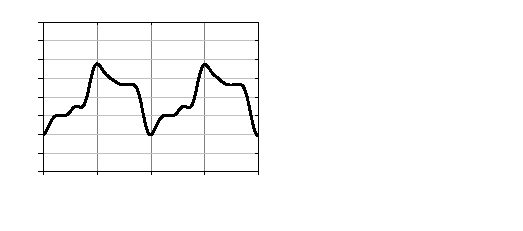
\includegraphics{meas_Output_CLoad_100M_1i0_3i0}
  \caption{
    Dashed line theoretical slope; solid black line measurement. Slope of (a) $\pm 1  i_0$ and (b) $\pm 3 i_0$.}
  \label{fig:meas_Output_CLoad_100M_1io_3io}
\end{figure}
% -----------------------------------------------------------------------------
The notation of both figures are the same, the solid black line represent the measured time domain signal for the frequency of 100 MHz, while the dashed line represent the theoretical signal waveform.

% ------------------------------------------------------------------------------
\section{Conclusion}
\label{sec:conclusion}
% ------------------------------------------------------------------------------
{\itshape
This letter presents a theory which considers second-harmonic losses in the
class-J PA mode. The theory predicts internal voltage waveforms, expressions
for power and efficiency and derives optimum fundamental impedances depending
on the second-harmonic loss. Load-pull measurements of a
6$\times$\SI{200}{\micro\meter} GaN HEMT device confirm the predicted waveforms
and validate the theoretical power and efficiency results. The theory may be
used to determine efficiency--bandwidth tradeoffs in wideband class-J PAs with
lossy second-harmonic loads.

}
% ------------------------------------------------------------------------------
% Appendices
% ------------------------------------------------------------------------------

\section*{Acknowledgement}
{\itshape
The authors would like to thank Thomas Maier at Fraunhofer IAF for carrying out
the load-pull measurements.
}

% ------------------------------------------------------------------------------
% References
% ------------------------------------------------------------------------------

%\bibliographystyle{IEEEtran}
%\bibliography{IEEEabrv,refs}

\end{document}

% EOF
